\subsection{Carnot Cycle}\label{subsec:Carnot_Cycle}
The \nameref{def:Process} path of the \nameref{def:Carnot_Cycle} is shown in \Cref{fig:Carnot_Cycle}.

\begin{figure}[h!tbp]
  \centering
  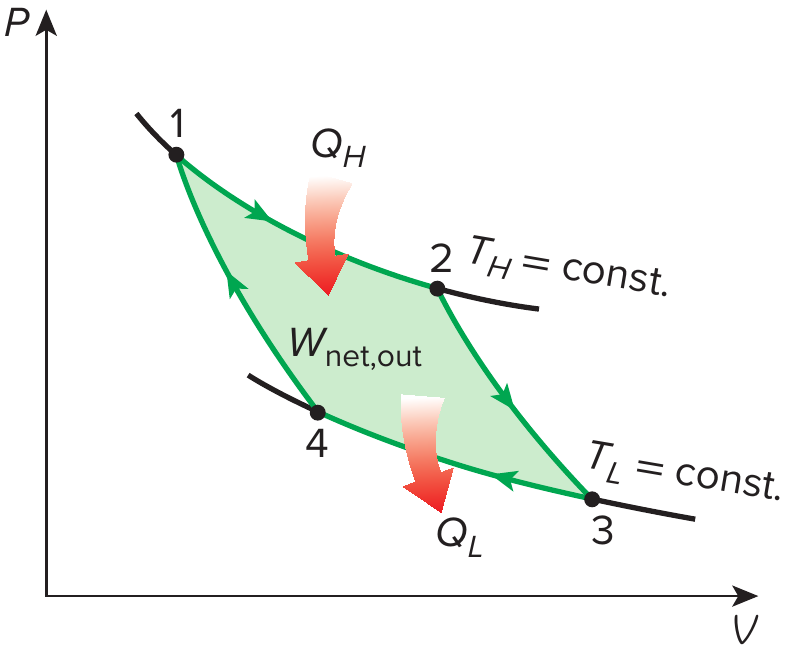
\includegraphics[scale=0.75]{Carnot_Cycle.png}
  \caption{Carnot Cycle (\cite[pg. 252]{ThermoTextbook})}
  \label{fig:Carnot_Cycle}
\end{figure}

\begin{definition}[Carnot Cycle]\label{def:Carnot_Cycle}
  The \emph{Carnot cycle} is a thermodynamically ideal \nameref{def:Cycle}.
  The temperatures $\Temp_{H}$ and $\Temp_{L}$ are isotherms.
  The vertical cases are times when the \nameref{def:System} is perfectly \nameref{def:Adiabatic}, meaning only \nameref{def:Work}, $\Work$, is done.
  The interior of the cycle's process path is the net work done by the \nameref{def:System}.
\end{definition}

If we look at the efficiency of the \nameref{def:Carnot_Cycle}, we see something interesting.
\begin{align*}
  \Efficiency_{C} &= 1 - \frac{\Heat_{Out}}{\Heat_{In}} \\
                  &= 1 - \frac{\Heat_{Out} \propto \Temp_{L}}{\Heat_{In} \propto \Temp_{H}} \\
                  &= 1 - \frac{\Temp_{L}}{\Temp_{H}}
\end{align*}

\begin{equation}\label{eq:Coefficient_of_Performance-Carnot_Cycle}
  \begin{aligned}
    \CoP_{C, HP} &= \frac{1}{1 - \frac{\Heat_{L}}{\Heat_{H}}} \\
    &= \frac{1}{1 - \frac{\Temp_{L}}{\Temp_{H}}} \\
  \end{aligned}
\end{equation}

Because the \nameref{def:Carnot_Cycle} is idealized, we can also run it backwards, making it a refrigerator.
This is seen in \Cref{fig:Carnot_Cycle-Backwards}.

\begin{figure}[h!tbp]
  \centering
  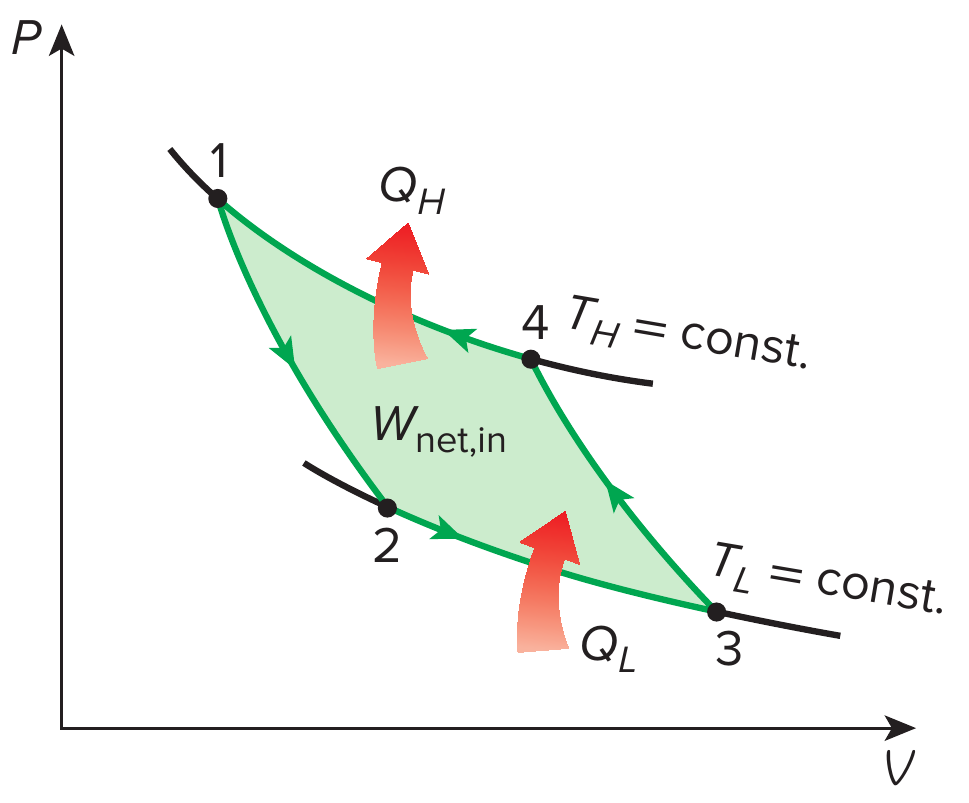
\includegraphics[scale=0.50]{Carnot_Cycle-Backwards.png}
  \caption{Carnot Cycle, in Reverse (\cite[pg. 253]{ThermoTextbook})}
  \label{fig:Carnot_Cycle-Backwards}
\end{figure}

The \nameref{def:Coefficient_of_Performance} for the reversed \nameref{def:Carnot_Cycle} is:
\begin{equation}\label{eq:Coefficient_of_Performance-Carnot_Cycle_Reversed}
  \begin{aligned}
    \CoP_{C, R} &= \frac{1}{\frac{\Heat_{H}}{\Heat_{L}} - 1} \\
    &= \frac{1}{\frac{\Temp_{H}}{\Temp_{L}} - 1} \\
  \end{aligned}
\end{equation}

\begin{remark*}
  For both \Cref{eq:Coefficient_of_Performance-Carnot_Cycle} and \Cref{eq:Coefficient_of_Performance-Carnot_Cycle_Reversed}, the temperatures \textbf{MUST} be in Kelvin or Rankine (\si{\kelvin}, \si{\rankine}).
\end{remark*}

\begin{example}[Textbook Problem 7.88]{Carnot Cycles on Power Plants}
  A geothermal power plant extracts geothermal water at $\Temp_{H} = \SI{160}{\degreeCelsius}$ at a rate of $\FlowRate{\Mass} = \SI{440}{\kilo\gram\per\second}$ as the heat source and produces $\FlowRate{\Work} = \SI{22}{\mega\watt}$ of power.
  If the environment temperature is $\Temp_{L} = \SI{25}{\degreeCelsius}$ determine the actual thermal efficiency, the maximum possible thermal efficiency, and the actual rate of heat rejection from the power plant?
  \tcblower{}
  \textbf{Concepts:} \\
  This is a power plant, so there must be a \nameref{def:Turbine}.
  We can refer back to \Cref{sec:Mass_Energy_Analysis_Control_Volumes} to help solve this.
  Namely,
  \begin{itemize}[noitemsep]
  \item $\FlowRate{\Work}_{Out}$ is large.
  \item $\FlowRate{\Work}_{In} \approx 0$
  \item $\FlowRate{\Heat} \approx 0$, meaning the turbine is adiabatic.
  \item $\Change{\KineticEnergy} = 0$
  \item $\Change{\Enthalpy} \neq 0$
  \end{itemize}

  We can also call this a \nameref{def:Carnot_Cycle}, where $\FlowRate{\Heat}_{H} = \FlowRate{\Heat}_{L} + \FlowRate{\Work}_{Out}$.
  In this case, the $\FlowRate{\Heat}_{H}$ is the water coming from the ground, the $\FlowRate{\Heat}_{L}$ is the atmosphere, and the $\FlowRate{\Work}_{Out}$ was provided. \\
  \begin{equation*}
    \begin{aligned}
      \Efficiency_{C} &= \frac{\FlowRate{\Work}_{Out}}{\FlowRate{\Heat}_{H}} \\
      &= 1 - \frac{\Temp_{L}}{\Temp_{H}}
    \end{aligned}
  \end{equation*}

  \textbf{Explore:} \\
  Because we weren't given any additional information about the input fluid, we assume that the fluid remains in a single state throughout the entire \nameref{def:Process}. \\
  For the \nameref{def:Turbine}, we have a mass flow that changes the energy balance.
  The energy balance is
  \begin{equation*}
    \FlowRate{\Heat}_{Net} - \FlowRate{\Work}_{Out} = \FlowRate{\Mass} (\SpecificEnthalpy_{Out} - \SpecificEnthalpy_{In})
  \end{equation*}

  $\FlowRate{\Heat}_{Net}$ means there is heat added and/or removed.
  If it is positive, then heat is being added.
  If it is negative, then heat is being removed. \\
  We can assume this fluid does not change state.
  We will also assume that hsi fluid is water, rather than steam.
  We can refer to Tables A.4 to find the specific enthalpies, because we have no pressures.

  \textbf{Plan:} \\
  Solve the \nameref{def:Turbine} energy balance. \\
  Solve the Carnot efficiency problem. \\
  The actual efficiency is $\Efficiency_{C} = \frac{\FlowRate{\Work}_{Out}}{\FlowRate{\Heat}_{H}}$.

  \textbf{Solve:} \\
  Solve for the net \nameref{def:Heat} for the \nameref{def:Turbine}.
  \begin{align*}
    \FlowRate{\Heat}_{Net} - \FlowRate{\Work}_{Out} &= \FlowRate{\Mass} (\SpecificEnthalpy_{Out} - \SpecificEnthalpy_{In}) \\
    \intertext{Finding the enthalpies from Table A.4.}
    \FlowRate{\Heat}_{Net} - \SI{22}{\mega\watt} &= \SI{440}{\kilo\gram\per\second} (104.8 - 675.5) \si{\kilo\joule\per\kilo\gram} \\
                                                    &= \SI{-251000}{\kilo\joule\per\second} \\
                                                    &= \SI{-251}{\mega\watt} \\
    \FlowRate{\Heat}_{Net} &= \SI{-229}{\mega\watt}
  \end{align*}

  The flowrate we found for the net heat from the turbine is negative, meaning the heat is flowing \textbf{out} of the turbine.

  Now, we find the heat the system rejects, $\FlowRate{\Heat}_{L}$.
  \begin{align*}
    \FlowRate{\Heat}_{L} &= \FlowRate{\Heat}_{H} - \FlowRate{\Work}_{Out} \\
                         &= \SI{229}{\mega\watt} - \SI{22}{\mega\watt} \\
                         &= \SI{251}{\mega\watt}
  \end{align*}

  We can now find the efficiency of the system.
  \begin{align*}
    \Efficiency_{Out} &= \frac{\FlowRate{\Work}_{Out}}{\FlowRate{\Heat}_{In}} \\
                    &= \frac{22}{251} \\
    &= 0.088
  \end{align*}

  We can now find the best case efficiency for the system using the efficiency of the \nameref{def:Carnot_Cycle}.
  \begin{align*}
    \Efficiency_{C} &= 1 - \frac{\Temp_{L}}{\Temp_{H}} \\
                    &= 1 - \SI{25}{160} \\
                    &= 0.312
  \end{align*}

  \textbf{Validate:} \\
  Double check our actual efficiency by solving
  \begin{equation*}
    \Efficiency_{Out} = 1 - \frac{\FlowRate{\Heat}_{L}}{\FlowRate{\Heat}_{H}}
  \end{equation*}

  \textbf{Generalize:} \\
  We had to consider two separate boundaries for the system.
  First was the \nameref{def:Turbine}'s boundary, the second was the \nameref{def:Carnot_Cycle} boundary.
\end{example}

\begin{example}[Textbook Problem 7.98]{Carnot Refrigerators}
  A Carnot \nameref{def:Refrigerator} removes \nameref{def:Heat} from a cool space at a rate of $\FlowRate{\Heat}_{L} = \SI{300}{\kilo\joule\per\minute}$ to maintain a temperature of $\Temp_{L} = \SI{-8}{\degreeCelsius}$.
  If the air surrounding the refrigerator is at $\Temp_{H} = \SI{25}{\degreeCelsius}$, determine the minimum power input, $\FlowRate{\Work}_{In}$, required by this refrigerator?
  \tcblower{}
  \textbf{Concepts:} \\
  A \nameref{def:Refrigerator} rejects heat from the interior (which it keeps cool) into the surroundings, in this case, the room.
  This heats up the room while keeping the inside of the fridge cool. \\
  If we model this as a \nameref{def:Carnot_Cycle}, we can find the \nameref{def:Coefficient_of_Performance} and the macroscopic energy flow.
  \begin{equation*}
    \FlowRate{\Heat}_{H} = \FlowRate{\Heat}_{L} + \FlowRate{\Work}_{In}
  \end{equation*}

  The \nameref{def:Coefficient_of_Performance} tells us how efficient the fridge is.
  If we relate it using the fact this refrigerator is a Carnot refrigerator, then we have this equation.
  \begin{equation*}
    \CoP_{C, R} = \frac{1}{\frac{\Temp_{H}}{\Temp_{L}} - 1}
  \end{equation*}

  Lastly, the $\CoP$ equation above is related to the work out by \Cref{eq:Coefficient_of_Performance-Refrigerator}.
  \begin{equation*}
    \CoP_{R} = \frac{\FlowRate{\Heat}_{L}}{\FlowRate{\Work}_{In}}
  \end{equation*}

  \textbf{Solve:} \\
  First, we find $\CoP_{C, R}$, remembering that the temperatures must be in absolute terms.
  \begin{align*}
    \CoP_{C, R} &= \frac{1}{\frac{\Temp_{H}}{\Temp_{L}} - 1} \\
                &= \frac{1}{\frac{25 + 273.15 \si{\kelvin}}{-8 + 273.15 \si{\kelvin}} - 1} \\
                &= 8.03
  \end{align*}

  Now, rearranging $\CoP_{R}$, we can solve for the \nameref{def:Work} in required.
  \begin{align*}
    \FlowRate{\Work}_{In} &= \frac{\FlowRate{\Heat}_{L}}{\CoP} \\
                          &= \frac{\SI{300}{\kilo\joule\per\minute}}{8.03} \\
                          &= \SI{32.63}{\kilo\joule\per\minute} \\
                          &= \SI{0.623}{\kilo\joule\per\second} \\
                          &= \SI{0.623}{\kilo\watt} \\
  \end{align*}

  \textbf{Validate:} \\
  This is a Carnot \nameref{def:Refrigerator} means that it is as efficient as possible, which explains the very low value of $\FlowRate{\Work}_{In}$ required.

  If the temperature outside the refrigerator is different, for example $\Temp_{H} = \SI{30}{\degreeCelsius}$, then the new $\CoP = 6.97$, making $\FlowRate{\Work}_{In} = \SI{0.717}{\kilo\watt}$.
  This means that the refrigerator requires more energy to cool the interior of the fridge compared to a cooler surroundings.
  This also makes sense because a hotter exterior means that more work must be put into keeping the interior cool.

  \textbf{Generalize:} \\
  The hotter the surroundings of the \nameref{def:Refrigerator}, the more inefficient it is. \\
  We solved for a Carnot refrigerator, which is the \textbf{most} ideal case, but a real refrigerator has inefficiencies.
\end{example}

\begin{example}[Textbook Problem 7.107]{Carnot Heat Pump}
  The structure of a house is such that it loses heat at a rate $\FlowRate{\Heat} = \SI{5400}{\kilo\joule\per\hour\per\degreeCelsius}$ between the indoors and outdoors.
  A \nameref{def:Heat_Pump} that requires an input of $\FlowRate{\Work}_{In} = \SI{6}{\kilo\watt}$ is used to maintain the house at $\Temp_{L} = \SI{29}{\degreeCelsius}$.
  Determine the lowest outdoor temperature in which the heat pump can meet the heating requirements of the house?
  \tcblower{}
  \textbf{Concepts:} \\
  The flowrate of heat looks a bit strange at first glance, but after looking at it for a little while, it starts to look familiar.
  \begin{equation*}
    \FlowRate{\Heat} = \frac{\FlowRate{\Heat}_{Out}}{\Change{\Temp}}
  \end{equation*}

  In addition, because the denominator is the change in temperature, in celsius, we can keep the number the same and treat it as the change in temperature in kelvin.
  \begin{equation*}
    \bigl( \SI{5400}{\kilo\joule\per\kilo\gram\per\kelvin} \bigr) (\Change \Temp) \si{\kelvin}
  \end{equation*}

  We were given very few details, so we have to take what we were given in a macroscopic view.
  Looking at the Carnot energy balance, we can see:
  \begin{equation*}
    \FlowRate{\Heat}_{H} = \FlowRate{\Heat}_{L} + \FlowRate{\Work}_{In}
  \end{equation*}

  We can view this \nameref{def:Heat_Pump} in two ways.
  The first is an idealized, Carnot depiction:
  \begin{equation*}
    \CoP_{C, HP} = \frac{1}{1- \frac{T_{L}}{T_{H}}}
  \end{equation*}

  The second is the realistic depiction:
  \begin{equation*}
    \CoP_{HP} = \frac{\FlowRate{\Heat}_{H}}{\FlowRate{\Work}_{In}}
  \end{equation*}

  \textbf{Explore:} \\
  For $\FlowRate{\Heat}_{L}$, the \nameref{rmk:Thermal_Reservoir} we will use is the air surrounding the hosue, rather than the earth.

  The value we were given was power per change in termperature.
  \begin{align*}
    \frac{\SI{5400}{\kilo\gram}}{\si{\hour} \Change{\Temp}} &= \frac{\SI{1.5}{\kilo\watt}}{\Change{\Temp}} \\
    \intertext{Let's keep everything in absolute temperatures until the very end.}
    &= \frac{\SI{1.5}{\kilo\watt}}{294.15 - \Temp_{L}}
  \end{align*}

  Now, we need to look at the \nameref{def:Coefficient_of_Performance}.
  \begin{align*}
    \CoP_{HP} &= \frac{\FlowRate{\Heat}_{H}}{\FlowRate{\Work}_{In}} \\
              &= \frac{1}{1 - \frac{T_{L}}{294.15}}
  \end{align*}

  \textbf{Plan:} \\
  Solve the \nameref{def:Coefficient_of_Performance} quadratic equation above.

  \textbf{Solve:} \\
  \begin{align*}
    \frac{\FlowRate{\Heat}_{H}}{\FlowRate{\Work}_{In}} &= \frac{1}{1 - \frac{\Temp_{L}}{294.15}} \\
    \Temp_{L} &= \SI{259.7}{\kelvin} \\
                                                       &= \SI{-13.3}{\degreeCelsius}
  \end{align*}

  \textbf{Validate:} \\
  To validate, we double-check by solving the \nameref{def:Coefficient_of_Performance} equation in the two different ways.
  \begin{align*}
    \CoP &= \frac{\frac{\SI{1.5}{\kilo\watt}}{294.15 - 259.7}}{\SI{6}{\kilo\watt}} \\
         &= 8.57 \\
    \CoP &= \frac{1}{1 - \frac{259.7}{294.15}} \\
         &= 8.57
  \end{align*}

  \textbf{Generalize:} \\
  An air \nameref{def:Heat_Pump} is limited in how low the exterior temperature can get before they become ineffective/inefficient.
\end{example}

\begin{example}[Textbook Problem 7.113]{Carnot Air Conditioner}
  An air conditioner with the refrigerant R-134a as a working fluid is used to keep a room at $\Temp_{L} = \SI{26}{\degreeCelsius}$ by rejecting the heat to the exterior at $\Temp_{H} = \SI{34}{\degreeCelsius}$.
  The room gains heat at a rate of $\Heat_{In} = \SI{50}{\kilo\joule\per\minute}$ while the room has $\Work_{In} = \SI{900}{\watt}$ of heat-generating components.
  The refrigerant enters the compressor at $\Pressure_{In} = \SI{500}{\kilo\pascal}$ as a \nameref{def:Saturated_Vapor} at a rate of $\FlowRate{\Volume} = \SI{100}{\liter\per\minute}$ and leaves at $\Pressure_{Out} = \SI{1200}{\kilo\pascal}$ and $\Temp_{Out} = \SI{50}{\degreeCelsius}$.
  Find the actual and the theoretical \nameref{def:Coefficient_of_Performance}, the minimum volume flowrate at the compressor?
  \tcblower{}
  \textbf{Concepts:} \\
  We are given the air conditioner with ``microscopic'' energy values/variables.
  However, we will need the macroscopic values to be able to calculate what we need to.

  Microscopic Variables:
  \begin{itemize}[noitemsep]
  \item State
  \item \nameref{def:Specific_Enthalpy}
  \item Actual $\FlowRate{\Work}_{In}$
  \end{itemize}

  Macroscopic Variables:
  \begin{itemize}[noitemsep]
  \item \nameref{def:Coefficient_of_Performance} modeled as a Carnot engine
  \item \nameref{def:Coefficient_of_Performance} modeled realistically
  \end{itemize}

  \textbf{Explore:} \\
  Because the compressor doesn't change anything other than the \nameref{def:Specific_Enthalpy} of a fluid, the energy balance is:
  \begin{equation*}
    \FlowRate{\Work}_{In} = \FlowRate{\Mass}(\SpecificEnthalpy_{Out}- \SpecificEnthalpy_{In})
  \end{equation*}

  To find the mass flowrate,
  \begin{equation*}
    \FlowRate{\Volume} = \FlowRate{\Mass} \SpecificVolume
  \end{equation*}

  Because the mass flowrate is constant, the \nameref{def:Specific_Volume} is constant, so $\SpecificVolume_{In} = \SpecificVolume_{Out} = \SpecificVolume$.

  To find the specific enthalpies, we use Tables A.11, A.12, and A.13.

  \textbf{Plan:} \\
  Solve for $\FlowRate{\Mass}$. \\
  Solve for $\FlowRate{\Work}_{In}$. \\
  Solve the \nameref{def:Coefficient_of_Performance} equation, both for the actual and the Carnot, using $\FlowRate{\Work}_{In} + \FlowRate{\Heat}_{L} = \FlowRate{\Heat}_{H}$.

  \textbf{Solve:} \\
  Starting with the inlet state, we are told it is a \nameref{def:Saturated_Vapor}, so:
  \begin{align*}
    \Quality &= 1 \\
    \Pressure_{In} &= \SI{500}{\kilo\pascal}
  \end{align*}

  So we use Table A.12.
  \begin{align*}
    \Temp_{Sat} &= \SI{15.7}{\degreeCelsius} \\
    \Vapor{\SpecificEnthalpy} &= \SI{259.3}{\kilo\joule\per\kilo\gram} \\
    \Vapor{\SpecificVolume} &= \SI{0.041118}{\meter\cubed\per\kilo\gram}
  \end{align*}

  Moving onto the outlet's state at $\Pressure_{Out} = \SI{1.2}{\mega\pascal}$ and $\Temp_{Out} = \SI{50}{\degreeCelsius}$, we see that the R-134a is a \nameref{def:Superheated_Vapor}.
  So, we use Table A.12.
  \begin{align*}
    \SpecificEnthalpy &= \SI{178.3}{\kilo\joule\per\kilo\gram} \\
    \SpecificVolume &= \SI{0.017301}{\meter\cubed\per\kilo\gram}
  \end{align*}

  Now, we can find the mass flowrate entering/leaving the compressor.
  \begin{align*}
    \FlowRate{\Volume} &= \FlowRate{\Mass} \SpecificVolume \\
    \FlowRate{\Volume} &= \SI{100}{\liter\per\minute} = 1.66 \times 10^{-3} \si{\meter\cubed\per\second} \\
    \FlowRate{\Mass} &= \frac{\FlowRate{\Volume}}{\SpecificVolume} \\
                       &= \SI{0.04053}{\kilo\gram\per\second}
  \end{align*}

  Now, we can find the \nameref{def:Work} required to compress the R-134a.
  \begin{align*}
    \FlowRate{\Work}_{In} &= \FlowRate{\Mass} (\SpecificEnthalpy_{Out}- \SpecificEnthalpy_{In}) \\
                          &= \SI{0.04053}{\kilo\gram\per\second} (278.3 - 259.3) \si{\kilo\joule\per\kilo\gram} \\
    &= \SI{0.7686}{\kilo\watt}
  \end{align*}

  We now find out the heat that is being added to the room.
  \begin{align*}
    \FlowRate{\Heat}_{L} &= \SI{250}{\kilo\joule\per\minute} + \SI{900}{\watt} \\
                         &= \SI{5.067}{\kilo\watt}
  \end{align*}

  Now, we can find the \nameref{def:Coefficient_of_Performance}, starting with the actual value.
  \begin{align*}
    \CoP_{AC} &= \frac{\FlowRate{\Heat}_{L}}{\FlowRate{\Work}_{In}} \\
              &= \frac{\SI{5.067}{\kilo\watt}}{\SI{0.7686}{\kilo\watt}} \\
    &= 6.59
  \end{align*}

  Now, for the idealized, maximum, \nameref{def:Coefficient_of_Performance}.
  \begin{align*}
    \CoP_{C, AC} &= \frac{1}{\frac{\Temp_{H}}{\Temp_{L}} - 1} \\
                 &= 37.4
  \end{align*}

  Because the Carnot version of this cycle is the most efficient, that means it will require the least power, and the least flowrate.
  \begin{align*}
    \Power_{Min} &= \FlowRate{\Work}_{In} \\
                 &= \frac{\SI{5.067}{\kilo\watt}}{37.4} \\
                 &= \SI{0.1356}{\kilo\watt} \\
    \intertext{The actual minimum power required is shown below.}
                 &= \SI{0.7686}{\kilo\watt}
  \end{align*}

  Now for the minimum flowrate required.
  \begin{align*}
    \FlowRate{\Mass} &= \frac{\FlowRate{\Work}_{In}}{\Change{\SpecificEnthalpy}} \\
                     &= \SI{0.007149}{\kilo\gram\per\second}
  \end{align*}

  Lastly, the volume flowrate required.
  \begin{align*}
    \FlowRate{\Volume}_{Min} &= \FlowRate{\Mass} \SpecificVolume \\
                             &= \SI{17.64}{\liter\per\minute}
  \end{align*}

  The mass flowrate out of the compressor is:
  \begin{align*}
    \FlowRate{\Mass}_{Out} &= \frac{\FlowRate{\Work}_{In}}{\Change{\SpecificEnthalpy}} \\
                           &= \SI{0.04}{\kilo\gram\per\second}
  \end{align*}
\end{example}

\subsubsection{Equating Carnot Efficiencies}\label{subsubsec:Equating_Carnot_Efficiencies}
We have 2 equations for the efficiency of a \nameref{def:Carnot_Cycle}.
\begin{align*}
  \Efficiency_{\text{Carnot}} &= \frac{\Temp_{H} - \Temp_{L}}{\Temp_{H}} = 1 - \frac{\Temp_{L}}{\Temp_{H}} \\
                              &= \frac{\Heat_{H} - \Heat_{L}}{\Heat_{H}} = 1 - \frac{\Heat_{L}}{\Heat_{H}}
\end{align*}

\paragraph{Reversible Carnot Cycles}\label{par:Reversible_Carnot_Cycles}
If we equate these (set them equal to each other) we get:
\begin{align*}
  1 - \frac{\Temp_{L}}{\Temp_{H}} &= 1 - \frac{\Heat_{L}}{\Heat_{H}} \\
  \frac{\Temp_{L}}{\Temp_{H}} &= \frac{\Heat_{L}}{\Heat_{H}} \\
  \frac{\Heat_{L}}{\Temp_{L}} &= \frac{\Heat_{H}}{\Temp_{H}} \\
  \frac{\Heat_{L}}{\Temp_{L}} - \frac{\Heat_{H}}{\Temp_{H}} &= 0
\end{align*}

This derivation's result is valid for any \nameref{def:Reversible_Process} which is a \nameref{def:Carnot_Cycle}.

%%% Local Variables:
%%% mode: latex
%%% TeX-master: "../../MMAE_320-Thermo-Reference_Sheet"
%%% End:
